\section{Hardware}
This section will describe and compare hardware that can be used to satisfy the conditions of the project.

\subsection{Specifications for NXT}
The LEGO Mindstorms NXT programmable robotics kit consists of various sensors, and a small computer which we shall hence forth call the NXT. The NXT consists of an ARM7 32-bit processor, 256kb of flash memory, 64kb of RAM and an 8-bit AVR microcontroller \cite{nxtspec}. The ARM CPU is used for general computations, and the AVR microcontroller is used to control the sensors and servo motors that can be connected to the NXT. The NXT also has a small LCD screen, Bluetooth support, a speaker, and can be connected to a computer through USB. It can take input from four sensors and control three motors at a time.

\subsubsection{ARM CPU}
The ARM family of chipsets are designed using the reduced instruction set computing (RISC) principles \cite{armarchitecture}. RISC processors generally use a small but optimized instruction set, and use the load/store architecture, which only allows memory to be accessed by load and store operations. ARM7 processors have a three stage pipeline. ARM processors differ from the regular x86 processors used in most personal computers in many ways. The shorter pipeline and smaller instruction set makes ARM processors much easier to predict, because of this it is also possible to optimize software for ARM processors much better than for x86 processors.

ARM processors are usually used in embedded systems such as cell phones, TVs, and most other consumer electronics. The reason for the ARM processors widespread use, is a relatively high performance at a low power consumption and a low price.

\subsubsection{Sensors}
In the NXT kit are servo motors that can be controlled by the NXT, these motors can be controlled in speed and degrees of rotation. The kit also includes touch sensors that can report if they are pressed or not.

An ultrasonic sensor is also included, this sensor can measure distance to an object, and detect movement. This is done by sending out ultrasonic sound waves that bounce off objects and are sent back. By measuring the time it takes for the sound waves to come back, the sensor can calculate the distance to the object. The object has to have a flat surface for the ultrasonic sensor to detect it.

\subsection{Specifications for Kinect}
An alternative to the ultrasound sensor is the Kinect from Microsoft. The Kinect is developed for the Xbox 360 to facilitate input without a typical controller. Instead the input is body movement from a person standing in front of the Kinect. The Kinect registers body movement by using a camera and an Infrared (IR) Depth Sensor \cite{kinectspec}. The regular RGB camera creates color images with a 1280x960 pixel resolution. The IR Depth Sensor works in combination with an IR Emitter that emits infrared light beams. The IR Depth Sensor reads these beams as they are reflected back from an object, measuring the distance between the object and the sensor. Both the RGB camera and the IR Depth Sensor has a 30 Hz refresh rate.

Even though the Kinect was designed to be used by the Xbox 360, a SDK for Windows have been released. The Kinect is thus capable of much more than finding people and their movements.

\subsection{LEGO Technic Competition Cannon}
It is difficult to build a cannon in LEGO, but we found a cannon that eliminates the need for us to build it. The Competition Cannon fits the LEGO that will be used to build the tower, while being able to produce reasonably precise and consistent shots.

\subsection{Preliminary tests}
To find the correct hardware to use, it is necessary to have information to make the correct decision. These tests include a comparison between the Kinect and the LEGO ultrasound sensor, and measurements of the precision of the LEGO Competition Cannon.

\subsubsection{Kinect \& LEGO ultrasound sensor}
When testing the Kinect and ultrasound sensor precision, we measured the distance to an object with a tape measure, and compared it to the distance reported from the sensors.

\autoref{fig:kinect-distance} shows the results from the Kinect testing, and \autoref{fig:ultrasound-distance} shows the result from the ultrasound sensor test.

\begin{figure}[hbtp]
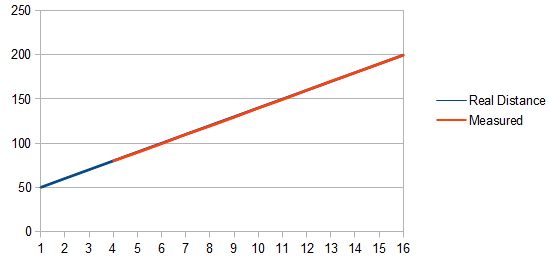
\includegraphics[width=\textwidth]{img/kinect-distance.png}
\caption{Kinect distance measurement.} 
\label{fig:kinect-distance} 
\end{figure}

\begin{figure}[hbtp]
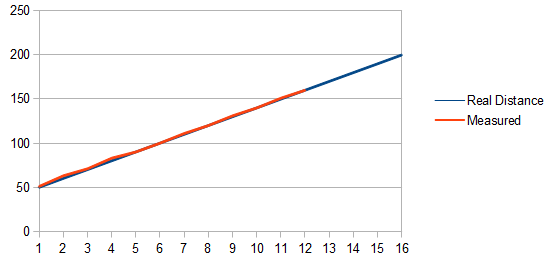
\includegraphics[width=\textwidth]{img/ultrasound-distance.png}
\caption{Ultrasound distance measurement.} 
\label{fig:ultrasound-distance} 
\end{figure}

The tests show that while the ultrasound sensor is a bit unprecise between 50 and 80 cm, the Kinect cannot measure closer than 80 cm, thus giving the ultrasound sensor an advantage.
On the other side of the spectrum, however, the ultrasound sensor cannot measure above 160 cm, while the Kinect can measure precisely at least up to our maximum distance measured of 200 cm.
Generally, the precision of both the ultrasound sensor and the Kinect is precise down to \textpm1 cm between 80 and 160 cm. The Kinect retains this precision up to at least 200 cm.

\subsection{Range of cannon}
The cannon's range has been measured by repeatedly shooting the cannon from specific angles, and calculating the average travel distance of the projectile from a specific angle. \autoref{fig:cannon-range} shows the average ranges from the measured angles.

These tests have been performed with the cannon at 80 cm above the ground.

\begin{figure}[hbtp]
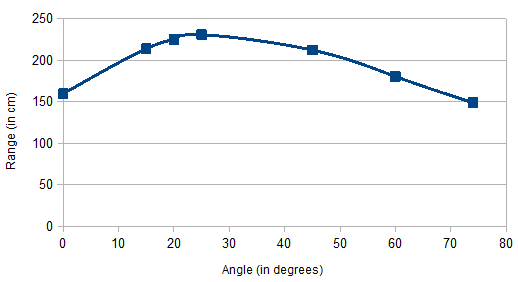
\includegraphics[width=\textwidth]{img/cannon-range.png}
\caption{The range of the cannon.} 
\label{fig:cannon-range} 
\end{figure}

We can gather from \autoref{fig:cannon-range} that the cannon shoots furthest at a 25 degree angle, where it shot the projectile a distance of 230 cm, and that shooting from 0 degrees gives the same result of 160 cm as shooting from 65 degrees. The results of the shots vary with a few centimeters in each direction from the average.

%\subsection{Choice of hardware}
%As we have easy access to the NXT, the use of it seems like the obvious choice. This means that the tower will also be built of LEGO, as the servo motors are built for this.

%The Competition Cannon has the ability to shoot in a range where both of our tested sensors can measure distance. The cannon is also precise enough that it should be possible to hit a moving target with it.

%Our central hardware choice is whether to use the supplied LEGO ultrasound sensor or the Kinect to measure distance. While the ultrasound sensor has the advantage of being able to measure distance to an object between 50 and 80 cm, it lacks ability in the upper distance range. The ultrasound sensor itself, however, is not enough to replace the Kinect. The ultrasound sensor can only measure distance to a single point, but to hit a moving object it is necessary to know both the speed and direction of an object as well as the distance to it. The Kinect does it all in one piece of hardware, for this reason, we will use the Kinect.